\documentclass{article}
\usepackage[utf8]{inputenc}
\usepackage{graphicx}
\usepackage{epstopdf}
\graphicspath{{./images/}}
\usepackage{caption}
\usepackage[english]{babel}
\usepackage{amsmath,amssymb,amsthm}
\usepackage{a4wide}
\usepackage{tikz}
\usetikzlibrary{calc}
\title{Analysis and Implementation of a Two-Scale Model for Dense Crowd Simulation}
\author{Omar Richardson\\Supervised by: Marko Boon, Adrian Muntean}
\let\oldhat\hat
\let\oldtil\tilde
\DeclareMathOperator{\diag}{diag}
\DeclareMathOperator{\D}{D}
\renewcommand{\vec}[1]{\mathbf{#1}}
\newcommand{\gvec}[1]{\boldsymbol#1}
\renewcommand{\tilde}[1]{\oldtil{\mathbf{#1}}}
\newcommand{\eps}{\varepsilon}
\newcommand{\bigo}[1]{\mathcal{O}\left(#1\right)}
\newtheorem{newdef}{Definition}
\newtheorem{newthm}{Theorem}
\begin{document}

\maketitle
\section{Abstract}
This report describes a crowd dynamics model [aggregated of microscale and macroscale][fitted for dense crowds]. [Implementation details][Implementation into software][results].
\newpage
\section{Introduction}
In this report, we present a novel implementation of a hybrid crowd dynamics model. Crowd dynamics studies the flow of pedestrians. Often, these studies are applied to specific situations, such as buildings, large scale events or traffic interaction. 
Since people are notably diverse and unpredictable, approaches in modelling and simulating pedestrians tend to vary a lot. 
Moreover, techniques in crowd dynamics do not only depend on the peoples' mindset, but also on their number, cultural habits, setting and perspective. 
To the authors knowledge, no model has yet been invented that applies on all situations of pedestrian interaction. 
However, since the late 20th century, a lot of progress has been made in developing and improving models that perform well in specific settings. 

\ \\
An intuitive way of modelling a crowd is by prescribing behavioural rules for each pedestrian that account for individual actions as well as interactions among them; this is considered a local approach.
However, this principle tends to scale poorly in the number of pedestrians. 
\ \\
For dense crowds, an alternative is to view the crowd as a whole, like a fluid or a gas. 
By prescribing a governing equation, together with an initial condition and boundary conditions, one obtains a global perspective of the flows and densities within the crowd. Hence, this is considered a global approach.
Global approaches have no description of individual pedestrian behaviour and therefore fail to adequately describe crowds with (regions of) low pedestrian density.

\ \\
An alternative is to combine both a local and global approach in a model, resulting in a \emph{hybrid} model. The local component is responsible for modelling individual preferences like goal or maximum speed, while the global component models the interaction between pedestrians.
Using the right simulation architecture, a hybrid model is able to simulate different type of crowds with a large number of agents at a relatively low computational cost.

\ \\
In this report, we propose and discuss a novel implementation based on Narain et al \cite{Narain04}.
 We provide a brief overview of the development of some of these models to provide a context for the model under consideration.
\newpage

\section{History}
Modelling crowds is a multidisciplinary field. While many early (and recent) models originate from mathematicians and physicists, large contributions have come from the computer science community as well, motivated by the need to create live-like environments for games and movies.
Also, scientists from the field of civil engineering and architecture have made major progress in development of crowd dynamic models, where one of the typical applications is ensuring and validating the safety standards of new constructions.
\paragraph{Particle models}
Perhaps the most popular way of modeling crowds is by prescribing the behaviour for each of the pedestrians individually.\\
While the idea sounds fairly intuitive, researchers have struggled with producing realistic and crowd-like motions. One of the first succesful attempts can be attributed to Reynolds in the late eighties \cite{Reynolds88}. In his attempt to model flocks of animals (specifically birds), he establishes rules which apply for many coherent groups of agents, including pedestrians. He proposes the Boid model (acronym for bird-oids, agents with birdlike flock behaviour) based on the principles of collision avoidance, velocity matching and flock centering.
\ \\
Reynolds main contribution is modelling a flock as a group of conforming agents, instead of individuals, and both reseachers as designers used these principles as a basis for realistic crowd motion.\\
However, in these models it is difficult to express individual preferences or characteristics. To resolve this, some researchers started to model crowds in a more physical setting, by applying kinematic principles to these agents, essentially treating them as particles.

\ \\
An influential example is Helbing's social force model \cite{Helbing98}, in which the pedestrians are represented as particles with a fixed mass and size.
These pedestrians have a preset goal, and try to reach that goal while maintaining their desired speed. While approaching the goal, they experience \emph{attraction} and \emph{repulsion} forces from other pedestrians and objects, depending on their personal preference. This way, both social behaviour is simulated as well as collision avoidance. 
Correctly implemented, this model shows realistic motions for the pedestrians. In addition, the model is able to capture crowd phenomena like lane formation and congestion. 
\ \\
This method has some drawbacks with respect to computations. While computing new pedestrian locations is linear in the number of pedestrians, computing the interaction forces scales quadratically, which is funest for large crowds.
\ \\
\paragraph{Continuum models}
When crowds become large, it may be convenient to model them on a macroscopic level. Among other earlier researchers, Henderson \cite{Henderson74} proposes a fluid-based crowd simulation. The individual masses and velocities of each pedestrian are converted to a global density and velocity field, and the evolution of this fluid-like crowd is computed using the Maxwell-Boltzmann transport equation. 

\ \\
Hughes describes a rather complete continuum theory of pedestrian flows in \cite{Hughes99}. His theory is based on the continuity equation but is complemented with a potential function for modelling discomfort at high densities. Walls, entrances and exits are modelled by prescribing at those locations respectivily fluxes, source terms, or sink terms.
\ \\
Hughes shows this model has a stable solution for densities within a certain interval. However, while these equations are able to model both subcritical (low-density) flows and supercritical (high density) flows, they fail to model situations in between.

\newpage
\section{Model}
We implement a hybrid model largely based on \cite{Narain04}.
In this model, two popular crowd simulation techniques are combined. On one hand, we will model the crowd as a system of interacting particles subject to external forces, as proposed by Helbing \cite{blabla}. 
In these types of models, referred to as \emph{particle models}, it is assumed each particle has a fixed set of goals and is attracted to these goals, while simultaneously evading obstacles and other pedestrians.

\ \\
Modelling pedestrians as particles lets us evaluate the crowd at microscale and allows us to model interaction and collision avoidance.
Figure \ref{fig:particle_model} shows an example of [particles with velocities]. These models are discrete in time, but continuous in space. For each particle $a$ with position $\vec{x}_a(t)$ and velocity $\vec{v}_b(t)$ at time $t$, we compute the position in the next time step $t+dt$ using the equation of motion:
\begin{equation}
	\vec{x}_a(t+dt) = \vec{x}_a(t) + \vec{v}_a(t)dt
	\label{(t)}
\end{equation}
\begin{figure}[h!]
	\centering
	\includegraphics[width=0.5\textwidth]{images/particles.pdf}
	\caption{Crowd representation by moving particles}
	\label{fig:particle_model}
\end{figure}
\\
On the other hand, we will model the crowd as a continuum, subject to the same laws (of nature) that apply to fluids. 
These models do not describe the motions of individual pedestrians, but rather the flow of the crowd as a whole. Because crowds are as diverse as the people of which they consists, there is not one unformly correct model. Succesful models were constructed around the Maxwell-Boltzmann equation \cite{Henderson77} and the continuity equation for the conservation of mass \cite{Hoogendoorn15}.
Our continuum model is based on the latter. 

\newpage
We apply the continuity equation augmented with a term accounting for pressure \eqref{eq:cont_equation}. We will impose group velocity $\vec{v}$ on individual pedestrians and apply a repulsive force from locations where the density $\rho$ is too high by introducing a pressure $p$.
\begin{equation}
	\frac{\partial\rho}{\partial t} = - \nabla \cdot (\rho\vec{v})+\nabla\cdot(\rho\nabla p).
	\label{eq:cont_equation}
\end{equation}
We will approximate this PDE on a fixed grid, so that we discretize in both time and space. Figure \ref{fig:cont_illustration} shows how this information can be represented.
\begin{figure}[h!]
	\centering
	\includegraphics[width=\textwidth]{images/continuum.pdf}
	\caption{Crowd representation in a corridor by density ($\rho$) and velocity fields ($\vec{v}$). The geometry and plots were made using this simulation.}
	\label{fig:cont_illustration}
\end{figure}
\\
Modelling the crowd as a continuum allows us to incorporate group behaviour.
\ \\
To unite these models, we obtain a continuous representation of the discrete particles, use that representation for our continuum model, and provide a way to impose the continuous information back to the particles. Elaboration on these steps is found in Section \ref{sec:continuum}.

\newpage
\section{Implementation}
The contributions in \cite{Narain04} only prescribes pedestrian movement and interaction. It has to be embedded in a particle model. The pedestrians in this model require knowledge of their surroundings and the ability to use that knowledge to find a path to their goal.
From this, we obtain the following demands: we need (1) to simulate arbitrary ortogonal geometries, (2) to provide agents with a goal and a (indicative) path towards that goal and (3) to convert pedestrians to a continuous representation. These requirements are worked out in this section.

\ \\
We implement this model in Python. This programming language has reliable scientific computing libraries available, like \texttt{numpy} and \texttt{scipy}. It also provides an object oriented structure, which makes description and manipulation of pedestrians on a local level more manageable.
\ \\
However, using pure Python can be quite slow in comparison to other (compiled) languages. For this reason, most of the computational intensive parts are (whenever possible) performed in the \texttt{numpy} library, which uses optimized C and FORTRAN code. This sharply reduces computational overhead.
\paragraph{Pedestrians}
As stated before, we model pedestrians as point particles with a fixed radius $r$ and mass $m$. Each pedestrian has a maximum speed $s$, randomly drawn from a set $[s_{\min},s_{\max}]$.
\paragraph{Geometry}
Simulation takes place in a rectangular domain of arbitrary size called a \emph{scene}.
At the start of the simulation, pedestrians are generated inside the free space of the scene, provided with a path that leads them to the exit.

\ \\
Within the scene, we define \emph{obstacles} as inaccesible static rectangular objects. One obstacle can connect to and even overlap another obstacle as to construct more general shapes. Pedestrians are able to assume any position where no obstacle is present.
 \\
By default, the scene is surrounded by a wall. Pedestrians are only able to escape the scene by walking through an \emph{exit}. In this implementation, we will restrict ourselves to a single exit per scene, but the simulation can easily be extended to multiple exits.

\paragraph{Visualization}
We add a graphical component to visualize the scene. This component displays the geometry and the pedestrians positions on each time step, as well as the continuum representation. We represent the continuum by plotting the discretization of density $\rho$, velocity field $\vec{v}$ and pressure $p$. Figure \ref{fig:example_scene} shows an example geometry filled with pedestrians. Figure \ref{fig:example_plot} shows the corresponding continuum plot. 
The visual component tries to provide a simple and schematic overview of the scene and the crowd without putting too much load on the CPU. However, graphical output can be supressed to increase computational capacity.
[We implement these parts in different modules, all disjunct]. [Also these methods are agnostic of each other].
\newpage

\section{Global planner}
This section describes the global planner module. The planner has the objective of planning a path for every agent to follow that will lead him to his goal. This path has to avoid the obstacles in the scene but ignores the position of other agents. Possible collisions with other agents will be avoided by the continuum solver. We elaborate on this module in Section \ref{sec:continuum}.

\ \\
In this implementation, we combine line segments to form piecewise linear paths. The path taken is the shortest path to the exit avoiding the obstacles. An example of a planned agent path is provided in Figure \ref{fig:example_path}. We compute a path by representing the scene as a weighted graph and determining the shortest path from the agents position to the exit.
\begin{figure}[h]
	\centering
	\includegraphics{images/example_graph.png}
	\caption{An example of a scene geometry and a indicative path from a pedestrians position to a goal.}
	\label{fig:example_path}
\end{figure}
\subsection{Graph representation}
We explain the planning algorithm by example. We model our scene as a two-dimensional set $\Omega \subset \mathbb{R}^2$. The scene contains $N_M$ obstacles $\{M_1,\dots,M_{N_M}\}$, and is initialized with $N_a$ agents with locations $(x_{a_j},y_{a_j}) \in \Omega$ for $j \in \{1,\dots,N_a\}$. 
\begin{newdef}
	Let $M \subset \Omega$ be a rectangular obstacle with lower left corner $\vec{s}=(s_x,s_y)$ and upper right corner $\vec{t}=(t_x,t_y)$. The shape of this obstacle is denoted as $[\vec{s},\vec{t}]$. The four corner points (lower-left, lower-right, upper-left and upper-right) are denoted respectivily as $\vec{m}^{00},\vec{m}^{10},\vec{m}^{01},\vec{m}^{11}$ and have values
	\begin{align}
		\vec{m}^{00}&=(s_x,s_y)\\
		\vec{m}^{10}&=(t_x,s_y)\\
		\vec{m}^{01}&=(s_x,t_y)\\
		\vec{m}^{11}&=(t_x,t_y)
		\label{eq:corner_points}
	\end{align}
\end{newdef}
Figure \ref{fig:example_path} shows an illustration of a scene $\Omega$ of size $R_x\times R_y$ containing $N_o = 2$ obstacles $M_1$ and $M_2$ with shapes $[\vec{s}_{M_1},\vec{t}_{M_1}]$ and $[\vec{s}_{M_2},\vec{t}_{M_2}]$. We seek a path for agent $a$ at location $\vec{x}_a$ to the exit $E$.

\ \\
Let $G = (V,A)$ be a weighted, undirected graph. 
Our vertex set $V$ is constructed by joining the set of all corner points with the pedestrian location and the exit.
\begin{equation}
	V = \left\{\left.\vec{m}^{ij}_k \right| i,j \in \{0,1\}, k = 1,\dots,N_o \right\} \cup \{E,a\}
	\label{eq:vertex_set_construction}
\end{equation}

\ \\
For each two nodes $v_i,v_j\in V$ we add edge $(v_i,v_j)$ to edge set $A$ if and only if the line segment between these points is contained in $\Omega$ and unhindered by other obstacles. The algorithm used to deduce whether a path is free of obstacles is described in Section \ref{sec:crosses_obstacle}. We choose the weight of the edge equal to the distance between the nodes. The result is a graph as depicted in Figure \ref{fig:example_graph}.

\ \\
We model the exit obstacle as a single node. The distance between an obstacle corner point and the exit is computed as the distance between a point and a set. This is motivated by wanting the pedestrians to find the fastest way to leave the scene. Also, we do not want to restrict their paths to the corners of the exit.
\begin{figure}[h]
	\centering
	\includegraphics[width=0.7\textwidth]{images/obstacle_graph.pdf}
	\caption{Example of the weighted graph corresponding to the scene in Figure \ref{fig:example_path}. The unmarked nodes correspond to the corners of the obstacles.}
	\label{fig:example_graph}
\end{figure}\\
Figure \ref{fig:example_graph} depicts the complete graph representation of the scene. Now, any path from node $\vec{x}_a$ to exit $E$ is a feasible path free of obstacles, since the edges are not hindered by obstacles.

\ \\
After obtaining this graph, we apply the $A^*$-algorithm to the graph to find the shortest path from $\vec{x}_a$ to $E$ and store it.
\newpage
\subsection{Determining hindering obstacles}
\label{sec:crosses_obstacle}
To find whether a line segment is free of obstacles, we use some basic linear algebra. Specifically, we use hyperplanes and \emph{bounding rectangles}. 
\ \\
First, some definitions:
\begin{newdef}
	Let $\Omega \in \mathbb{R}^2$ be a scene.
	Let $l\subset \Omega$ be a line segment from $\vec{p}$ to $\vec{q}$ with $\vec{p},\vec{q} \in \mathbb{R}^2$. Then the corresponding hyperplane $L$ (i.e., the hyperplane that covers the line segment) is defined as the set of all $\vec{x}\in\mathbb{R}^2$ satisfying
	\begin{equation}
		(\vec{a},\vec{x})=b
	\end{equation}
	where $\vec{a}$ and $b$ equal 
	\begin{align}
		\vec{a} &= \left( -(p_y-q_y),(p_x-q_x)\right)\\
		b   &=  p_y(p_x - q_x) - p_x(p_y - q_y)
	\end{align}
\end{newdef}
\noindent
A hyperplane separates the set $\Omega$ into two sets $\Omega_{L^+}$ and $\Omega_{L^-}$ such that
\begin{align}
\Omega = \Omega_{L^+} \cup \Omega_{L^-} \cup L\\
\Omega_{L^+}\cap\Omega_{L^+}=\emptyset.
	\label{def:hyp}
\end{align}
It is a simple task to determine whether a point $\vec{x}$ belongs to either one of the subsets (or the hyperplane itself) by computing the inner product with $\vec{a}$.
\begin{newdef}
	Let $\vec{x}$ be a point in $\mathbb{R}^2$. Let $L$ be a hyperplane separating $\Omega$ into subsets $\Omega_{L^+}$ and $\Omega_{L^-}$. These sets are defined in the following way:
	\begin{equation}
		\begin{cases}
			\vec{x} \in L&\mbox{ if }(a,x) = b\\
			\vec{x}  \in \Omega_{L^-} &\mbox{ if }(a,x) < b\\
			\vec{x}  \in \Omega_{L^+} &\mbox{ if }(a,x) > b\\
		\end{cases}
		\label{eq:separation}
	\end{equation}
\end{newdef}
\begin{newdef}
	Let $l$ be a line segment from $\vec{p}$ to $\vec{q}$. The bounding rectangle $P_l$ is defined as the smallest rectangle containing $l$:
	\begin{equation}
		P_l = \left\{ w\in\mathbb{R}^2| \min\{p_x,q_x\} \leq w_x \leq \max\{p_x,q_x\}, \min\{p_y,q_y\} \leq w_y \leq \max\{p_y,q_y\}  \right\}
		\label{eq:bounding_rect}
	\end{equation}
\end{newdef}
\noindent
An example of a bounding rectangle is illustrated in Figure \ref{fig:bounding_rect_ex}.
\begin{figure}
	\centering
	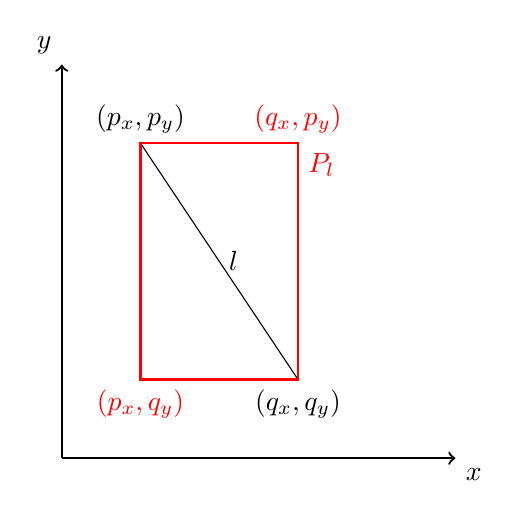
\begin{tikzpicture}
		\draw[step=2cm,black,thin] (1,4) node[anchor=south] {$(p_x,p_y)$} -- node[anchor=west]{$l$} (3,1) node[anchor=north] {$(q_x,q_y)$};
		\draw[thick,red] (1,1) rectangle (3,4) node[anchor=north west]{$P_l$};
		\draw[step=2cm,black,thin] (1,1) node[anchor=north,red] {$(p_x,q_y)$};
		\draw[step=2cm,black,thin] (3,4) node[anchor=south,red] {$(q_x,p_y)$};
		\draw[thick,->] (0,0) -- (5,0) node[anchor=north west] {$x$};
		\draw[thick,->] (0,0) -- (0,5) node[anchor=south east] {$y$};
	\end{tikzpicture}
	\captionof{figure}[Caption]{Line segment $l$ and the corresponding bounding rectangle $P_l$ with shape $[(p_x,q_y),(q_x,p_y)]$}
	\label{fig:bounding_rect_ex}
\end{figure}

\begin{newthm}
	Let $A$ and $B$ be two rectangles with shapes $[\vec{s}_A,\vec{t}_A]$ and $[\vec{s}_B,\vec{t}_B]$. Then the intersection $A\cap B$ is non-empty if and only if
	\begin{equation}
		\vec{t}_{Ai} < \vec{s}_{Bi} \mbox{ or }	\vec{t}_{Bi} < \vec{s}_{Ai}\, \forall i \in \{1,2\}
		\label{eq:intersection}
	\end{equation}
	\label{thm:intersect}	
\end{newthm}
\begin{newthm}
	Let $l\subset \Omega$ be a line segment and $M \subset \Omega$ be an obstacle. Then the following statements are equivalent:
		\begin{enumerate}
			\item $l \cap M = \emptyset$
			\item $P_l \cap M = \emptyset \mbox{ or } M \subset \Omega_{L^+} \mbox{ or } M \subset \Omega_{L^-}$
		\end{enumerate}
	\label{thm:sep}
\end{newthm}
\begin{proof}
	(2) $\implies$ (1):\\
	Assume $P_l \cap M = \emptyset$. We know $l \subset P_l$ and therefore $l \cap M = \emptyset$.\\
	Otherwise, without loss of generality, assume $M \subset \Omega_{L^+}$. We know $\Omega_{L^+} \cap l = \emptyset$ so $M \cap l = \emptyset$.

	\ \\
	$\neg (2) \implies \neg (1)$:\\
	Assume $P_l \cap M \neq \emptyset,\, M \not\subset \Omega_{L^+} \mbox{ and } M \not\subset \Omega_{L^-}$.\\
	Let $C := P_l \cap M$. $C$ is the intersection of two rectangular sets and therefore rectangular itself.\\
	Let $C^+:=P_l \cap M \cap \Omega^{L^+}$ and $C^-:= P_l \cap M \cap \Omega^{L^-}$. By construction (\emph{needs more argument}), we know $C^+$ and $C^-$ are non-empty sets.
	
	\ \\
	We can pick $\vec{c}^+ \in C^+$ and $\vec{c}^- \in C^-$ and construct line segment $c$ from $\vec{c}^+$ to $\vec{c}^-$. Since $C^+,C^- \subset C$ and $C$ is a convex set, we know $c \subset C$. But since $\vec{c}^+ \in \Omega_{L^+}$ and $\vec{c}^- \in \Omega_{L^-}$ we know $c$ intersects $l$, so $l \cap M \neq \emptyset$.
\end{proof}
\newpage
\noindent
Based on Theorem \ref{thm:intersect} and \ref{thm:sep}, we obtain an computationally efficient way to determine the obstacles crossing a line segment.
Figure \ref{fig:crosses_obstacle} depicts an example of an obstacle and a line segment which do not intersect.
Since a rectangle is a convex set, checking $M \subset A$ reduces to checking $\vec{m}^{ij} \in A$ for $i,j \in \{0,1\}$.
\emph{Maybe say something about the efficiency of the calculation}
\\ \
\begin{figure}[ht]
	\centering
	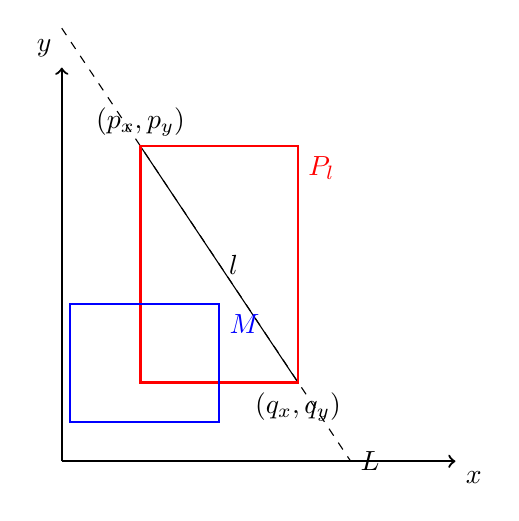
\begin{tikzpicture}
		\draw[step=2cm,black,thin] (1,4) node[anchor=south] {$(p_x,p_y)$} -- node[anchor=west]{$l$} (3,1) node[anchor=north] {$(q_x,q_y)$};
		\draw[step=2cm,black,thin,dashed] (0,5.5) -- (3.67,0) node[anchor=west]{$L$};
		\draw[thick,red] (1,1) rectangle (3,4) node[anchor=north west]{$P_l$};
		\draw[thick,blue] (0.1,0.5) rectangle (2,2) node[anchor=north west]{$M$};
		\draw[thick,->] (0,0) -- (5,0) node[anchor=north west] {$x$};
		\draw[thick,->] (0,0) -- (0,5) node[anchor=south east] {$y$};
	\end{tikzpicture}
	\captionof{figure}[Caption]{Line segment $l$ and obstacle $M$. There is a non-empty intersection between $P_l$ and $M$, but no intersection between $l$ and $M$ because all of $M$ lies on the same side of the hyperplane $L$.}
	\label{fig:crosses_obstacle}
\end{figure}\\
\newpage
\section{Continuum aspects}
\label{sec:continuum}
This section will elaborate on the continuum part of the implementation; converting the agents to a continuum and computing its properties.
\subsection{Overview}
The \underline{continuum solver} uses the following partial differential equation, based on the continuity equation for mass but adapted with a pressure term.
\begin{equation}\label{eq:pde}
\frac{\partial \rho}{\partial t} =-\nabla \cdot(\rho{v}) + \nabla \cdot (\rho\nabla p)
\end{equation}
with scalar density field $\rho(x,y,t)$, vector velocity field $v(x,y,t) = \begin{pmatrix}v_x\\v_y\end{pmatrix}$ and scalar pressure field $p(x,y,t)$.

\ \\
To utilise our fluid flow solver, we need a global representation of the agents. The agents' individual mass and velocity has to be converted to a global density, velocity and pressure. In this implementation, we choose to define a grid of cells over the scene. In each cell, we compute a numerical estimate for each field. Both the density and the velocity of a given cell are interpolated from the agents nearby the cell. Then, using these two fields, we numerically compute the next time step of the pressure and the velocity in \eqref{eq:pde}. Finally, we use these two fields to restrict the motion of the agents.

\ \\
Our fluid solver influences the agents in two ways: 
\begin{itemize}
\item Swarm behaviour
\item Incompressibility
\end{itemize}
\subsubsection{Incompressibility Constraint}
Our incompressibility imposes some restrictions on the density and the velocity. We assume a maximum density $\rho_{\max}$. Wherever our density $\rho(x)$ reaches $\rho_{\max}$, the scene is locally saturated, and the agents have to divert from their path. 

\ \\
\underline{Using variational calculus} we obtain that the optimal $v$ respecting $v_{\max}$ equals $$v = v_{\max}\frac{v-\nabla p}{||v-\nabla p||}.$$
under the constraints that 
\begin{align}
\label{eq:comp}
p>0 \texttt{ OR } \rho=\rho_{\max}\\
p>0 \implies \nabla\cdot v=0
\end{align}
Note that \eqref{eq:comp} implies that $\rho$ and $p$ are complementary variables, i.e. that $\rho(x)p(x)=0$ for all $x$.
\subsubsection{Swarm behaviour}
The solver computes the velocity field of the crowd on a grid. This field influences the individual speed of the agents. When the density in an agents neighbourhood becomes higher, his velocity will converge to the velocity of the crowd. The actual velocity $v_{a_i}$ of agent $a_i$ (located at $(x_{a_i},y_{a_i})$) becomes the average of his desired velocity $\bar{v}_{a_i}$ and the crowds velocity $v(x_{a_i},y_{a_i},\cdot)$, weighted to the local density:
\begin{equation}
	v_{a_i} = \left(1-\frac{\rho(x_{a_i},y_{a_i},\cdot)}{\rho_{\max}}\right)\bar{v}_{a_i}+\frac{\rho(x_{a_i},y_{a_i},\cdot)}{\rho_{\max}}v(x_{a_i},y_{a_i},\cdot)
	\label{eq:dens_velo}
\end{equation}


\subsection{Discretization}
We require a numerical approximation of $\rho$, $p$ and $v$. To obtain this, we first discretize our domain and our equation. We define a grid of $(N_x,N_y)$ cells, where every cell has a size of $h_x\times h_y$. Our complete scene has dimensions $N_xh_x\times N_yh_y$. 
\ \\
We discretize our scalar and vector fields corresponding to the grid. We index the cells (and the fields) from the bottom left, corresponding with the Carthesian coordinate system in the scene. This is illustrated in Figure \ref{fig:indexing}.
\begin{figure}
	\centering
	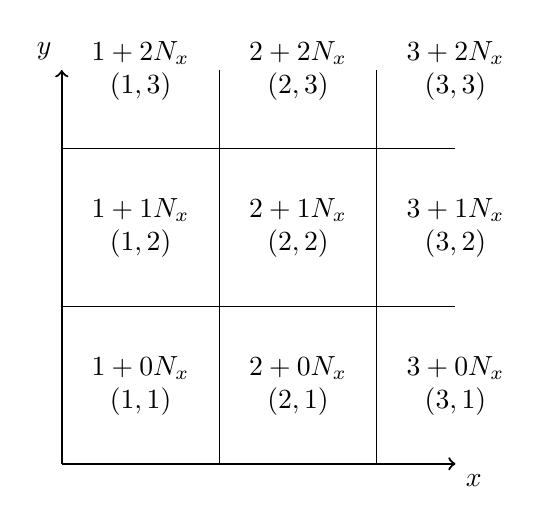
\begin{tikzpicture}
		\draw[step=2cm,black,thin] (0,0) grid (5,5);
		\draw[thick,->] (0,0) -- (5,0) node[anchor=north west] {$x$};
		\draw[thick,->] (0,0) -- (0,5) node[anchor=south east] {$y$};
		\foreach \x in {1,2,3}
			\pgfmathparse{\x*2-1}
			\edef\cx{\pgfmathresult}
			\foreach \y in {1,2,3}
				\pgfmathparse{\y*2-1}
				\edef\cy{\pgfmathresult}
				\pgfmathparse{int(\y-1)}
				\edef\ym{\pgfmathresult}
				\draw (\cx cm,\cy cm) node[anchor=center] {$\begin{matrix}\x+\ym N_x\\ (\x,\y)\end{matrix}$};
	\end{tikzpicture}
	\captionof{figure}[Caption]{Orientation of the coordinates and fields in the scene, with corresponding $\left(\begin{matrix}\text{1D} \\ \text{2D} \end{matrix}\right)$ cell indexing of the scene. The 1D notation is used to orient corresponding vectors and matrices, while the 2D notation is used for legibility and elementwise computations}
	\label{fig:indexing}
\end{figure}
This way, we discretize our fields to vectors $\gvec{\rho}^n,\vec{v_x}^n,\vec{v_y}^n, \vec{p}^n\in\mathbb{R}^{N_xN_y}$ for any time step $n\in\mathbb{N}$. The relation between a field $u$ and its discrete representation $\vec{u}^n$ is defined as
$$\vec{u}^n_{(i,j)} = u((i-0.5)\Delta x,(j-0.5)\Delta y,n\Delta t)$$
This way the entries of vector $\vec{u}$ are approximations at the centre of the corresponding cells.
\ \\
So for any discrete scalar field $\vec{u}$, the value in cell $(i,j)$ is denoted as $\vec{u}_{i+(j-1)N_x}$. To increase legibility, we introduce a corresponding notation for indexing the scalar field in $(i,j)$:
\begin{equation}
	\vec{u}_{(i,j)}:=\vec{u}_{i+(j-1)N_x}
\end{equation}
\subsection{Interpolation}
Before being able to discretize our density and velocity fields, we first need to interpolate them from individual agent positions. Let the scene contain $n$ agents, $a_1,\dots,a_n$, located at position $(x_{a_i},y_{a_i})$.
\ \\
The agents are modelled as Lagrangian particles. This means the agents have no volume, but their mass and velocity are concentrated into a single point.
In this implementation, we assume equal mass for all agents: $m_{a_i}=m = 1\ \forall i$. 
We convert an agents mass to a density by convolving with a two-dimensional Gaussian kernel $\phi(x,y)$ defined as 
\begin{equation}
	\label{eq:gaussian}
	\phi(x,y)=A \exp\left(-\left(\frac{x^2}{2\sigma_x^2}+\frac{y^2}{2\sigma_y^2}\right)\right)
\end{equation}
\emph{Currently, we are in the process of finding suited values for $A$, $\sigma_x$ and $\sigma_y$.}

\ \\
Let $\delta_{(x_0,y_0})$ be the Dirac distribution with value $\infty$ in $(x_0,y_0)$ and 0 everywhere else. Let $f*g$ be the convolution of $f$ and $g$. 
\ \\
Let agent $a_i$ be in location $(x_{a_i},y_{a_i})$ at time $t$. Then the density contribution $\rho_{a_i}(x,y)$ and velocity contribution $v_{a_i}(x,y)$ become
\begin{align}
	\rho_{a_i}(x,y) = m\delta*\phi\\
	v_{a_i}(x,y) = \begin{pmatrix}v_{a_i,x}\\v_{a_i,y}\end{pmatrix}\delta*\phi
\end{align}
Since $\phi$ is rotation symmetric, it can be expressed in polar coordinates:
\begin{align}
	r = \sqrt{\frac{x^2}{2\sigma_x^2}+\frac{y^2}{2\sigma_x^2}}\\
	\phi(r) = A\exp\left(-r^2\right).
\end{align}
We use a approximation of the Gaussian kernel called the Wendland-kernel \cite{violeau12}. This kernel is defined as follows:
\begin{equation}
	\label{eq:wendland}
	f_W(r) = \begin{cases}
				\left(1-\frac{r}{2}\right)^4(1+2r)& 0\leq r \leq 2\\
				0 & 2 < r 
			\end{cases}
\end{equation}
This approximation has some nice computational properties in comparison to other Gaussian approximation. We can reveal them by rewriting the expression to 
\begin{equation}
	f_W(r) = \max\left\{1-\frac{r}{2},0\right\}^4(1+2r)
\end{equation}
which is a single case function requiring only addition, multiplication, and a $\max$ function. This provides a welcome computational benefit, since a kernel convolution is a common operation in this implementation.

\ \\
To find the total density and total velocity in the cell centres for each cell, we sum over the densities and velocities of the agents in the (up to 8) neighbouring cells. This method is equivalent to the particle-in-cell method as described in \cite{zhu13}.\\
\begin{figure}[h]
	\centering
	\includegraphics[width=0.65\textwidth]{images/scene.png}
	\caption{Scene initiated with 1000 agents being directed to the exit south}
	\label{fig:cont_ex_scene}
\end{figure}
\begin{figure}[h]
	\centering
	\includegraphics[width=0.85\textwidth]{images/flow_fields.png}
	\caption{Continuous representation of the scene: density and velocity}
	\label{fig:cont_flow_field}
\end{figure}\\
Figure \ref{fig:cont_ex_scene} shows an example scene with agents. Figure \ref{fig:cont_flow_field} shows the corresponding density and velocity fields.
\subsection{Scheme}
\label{sec:scheme}
To discretize our partial differential equation we use a second order central difference scheme. So for scalar field $u$ we have the following gradient approximation:
\begin{align*}
\nabla u=\begin{pmatrix}\dfrac{\partial u}{\partial x}\\\dfrac{\partial u}{\partial y}\end{pmatrix}
=\begin{pmatrix}\dfrac{\vec{u}_{(i+1,j)}-\vec{u}_{(i-1,j)}}{2h_x}\\\dfrac{\vec{u}_{(i,j+1)}-\vec{u}_{(i,j-1)}}{2h_y}\end{pmatrix}+\bigo{h^2}.
\end{align*}
and for vector field $w$ we define the divergence approximation accordingly:
\begin{equation}
\nabla\cdot w=\dfrac{\partial w}{\partial x}+\dfrac{\partial w}{\partial y}=\dfrac{\vec{w}_{(i+1,j)}-\vec{w}_{(i-1,j)}}{2h_x}+\dfrac{\vec{w}_{(i,j+1)}-\vec{w}_{(i,j-1)}}{2h_y}+\bigo{h^2}.
\end{equation}
However, if we were to discretize $\nabla\cdot(\nabla u)$ this way, computing the value at cell $(i,j)$ would require cell values from non-adjacent neigbour cells. Therefore, when computing the divergence of the gradient, we use the more compact scheme:
\begin{equation*}
\nabla\cdot(\nabla u) = \dfrac{\vec{u}_{(i+1,j)}-2\vec{u}_{(i,j)}+\vec{u}_{(i-1,j)}}{h_x^2}+\dfrac{\vec{u}_{(i,j+1)}-2\vec{u}_{(i,j)}+\vec{u}_{(i,j-1)}}{h_y^2}+\bigo{h^2}
\end{equation*}
This way, we have ensured all terms of the PDE can be computed for every cell not on the boundary.

\ \\
To discretize in time, we use the explicit Euler method. This way we only need the values of the previous time step to compute the values of the next time step. This suits our system best, because after every iteration of the fluid flow solver, the scene has changed due to individual actions of agents. Therefore previous time steps have little practical information.

\ \\
Our resulting scheme is presented below:
\begin{equation}
	\begin{split}
		\dfrac{\gvec{\rho}^{n+1}_{(i,j)} - \gvec{\rho}^{n}_{(i,j)}}{\Delta t} =
		% div(\gvec{\rho}*v)\Delta t
		&-\dfrac{\gvec{\rho}^{n}_{(i+1,j)}\vec{v}^{n}_{x(i+1,j)}-\gvec{\rho}^{n}_{(i-1,j)}\vec{v}^{n}_{x(i-1,j)}}{2h_x} \\
		&-\dfrac{\gvec{\rho}^{n}_{(i,j+1)}\vec{v}^{n}_{y(i,j+1)}-\gvec{\rho}^{n}_{(i,j-1)}\vec{v}^{n}_{y(i,j-1)}}{2h_y}\\
		%div(\gvec{\rho}*\grad \vec{p})\Delta t
		&+\frac{1}{h^2_x}\left(\frac{1}{4}(\gvec{\rho}^{n}_{(i+1,j)}-\gvec{\rho}^{n}_{(i-1,j)})(\vec{p}^{n}_{(i+1,j)}-\vec{p}^{n}_{(i-1,j)})+ \gvec{\rho}^{n}_{(i,j)}(\vec{p}^{n}_{(i+1,j)}-2\vec{p}^{n}_{(i,j)}+\vec{p}^{n}_{(i-1,j)})\right)\\
		&+\frac{1}{h^2_y}\left(\frac{1}{4}(\gvec{\rho}^{n}_{(i,j+1)}-\gvec{\rho}^{n}_{(i,j-1)})(\vec{p}^{n}_{(i,j+1)}-\vec{p}^{n}_{(i,j-1)})+ \gvec{\rho}^{n}_{(i,j)}(\vec{p}^{n}_{(i,j+1)}-2\vec{p}^{n}_{(i,j)}+\vec{p}^{n}_{(i,j-1)})\right)
	\end{split}
	\label{eq:scheme}
\end{equation}
It is suitable to express our scheme in terms of matrices and vectors. Not only does this provide us with an efficient way to implement our scheme, it also sets us up for an efficient way of solving the PDE (as explained in Section \ref{sec:lcp})

\ \\
Before reformulating our scheme, we introduce \emph{Kronecker} products and vector gradients.
\subsubsection{Kronecker product}
Let $A \in \mathbb{R}^{m\times n}$ and $B \in \mathbb{R}^{p \times q}$. The Kronecker product $A\otimes B\in \mathbb{R}^{mp \times nq}$ is defined as
\begin{equation*}
	A\otimes B = \begin{pmatrix}
		a_{11}B &\cdots & a_{1n}B\\
		\vdots & \ddots & \vdots\\
		a_{m1}B & \cdots & a_{mn}B
	\end{pmatrix}.
\end{equation*}
The Kronecker product will prove valuable in notation and computation of our matrices.
% \subsubsection{Hadamard Product}
% Let $A \in \mathbb{R}^{m\times n}$ and $B \in \mathbb{R}^{m \times n}$. The Hadamard product $A\circ B\in \mathbb{R}^{m \times n}$ is the elementwise product of $A$ and $B$:
% \begin{equation*}
% 	A\circ B = \begin{pmatrix}
% 		a_{11}b_{11} &\cdots & a_{1n}b_{1n}\\
% 		\vdots & \ddots & \vdots\\
% 		a_{m1}b_{m1} & \cdots & a_{mn}b_{mn}
% 	\end{pmatrix}.
% \end{equation*}
% Each of the terms \eqref{eq:scheme1}, \eqref{eq:scheme1}, \eqref{eq:scheme3}, and \eqref{eq:scheme4} can be expressed separately by a combination of Kronecker products.
\subsubsection{Vector difference operator}
In Section \ref{sec:scheme} we defined the discretization of the gradient. We would like to compute a gradient for every cell in the scene, even for the boundary. We introduce a directional \emph{difference operator} that will aid us in computing the gradient approximation. First we surround our scene with a extra layer of cells. These virtual cells are meant to ensure the presence of 8 neighbour cells for all the cells in the scene. We fix the density and velocity in these virtual cells to 0. 
For a discrete field $\vec{u}\in \mathbb{R}^{N_xN_y}$ let the auxiliary extended field be denoted by $\vec{\tilde{u}} \in \mathbb{R}^{(N_x+2)(N_y+2)}$ defined such that:
\begin{equation}
	\vec{\tilde{u}}_{(i,j)} = \begin{cases}
		\vec{u}_{(i,j)}&\mbox{if } i \in \left\{ 1,\dots,N_x \right\},j \in \left\{ 1,\dots,N_y \right\} \\
		0&\mbox{else}
	\end{cases}.
	\label{def:gradient}
\end{equation}
We define our difference operators $\D_x, \D_y:\mathbb{R}^{N_xN_y}\to\mathbb{R}^{N_xN_y}$ as follows:
\begin{align*}
	\left( \D_x\vec{u} \right)_{(i,j)} &= \vec{\tilde{u}}_{(i+1,j)}-\vec{\tilde{u}}_{(i-1,j)}\\
	\left( \D_y\vec{u} \right)_{(i,j)}  &= \vec{\tilde{u}}_{(i,j+1)}-\vec{\tilde{u}}_{(i,j-1)}
	%&\forall i\in \left\{ 1,\dots,N_x \right\},\,\forall j \in \left\{ 1,\dots,N_y \right\}
\end{align*}
\subsubsection{Matrix composition}
We first define two tridiagonal matrices $P_{m},Q_{m}\in \mathbb{R}^{m\times m}$
\begin{align*}
	P_{m} &= \begin{pmatrix}
		0 & 1 &  & &  \\
		-1 & 0 & 1 &   &  \\
		  & -1 & \ddots & \ddots &  \\
		  &  & \ddots & \ddots &1 \\
		 & &  & -1 & 0
	\end{pmatrix}\\
	Q_{m} &= \begin{pmatrix}
		-2 & 1 &  & &  \\
		1 & -2 & 1 &   &  \\
		  & 1 & \ddots & \ddots &  \\
		  &  & \ddots & \ddots &1 \\
		 & &  & 1 & -2
	\end{pmatrix}
\end{align*}
Let $I_m$ be the identity matrix of rank $m$. Let $\diag:\mathbb{R}^n\to\mathbb{R}^{n\times n}$ be the operator that converts a vector $\vec{p}$ to a diagonal matrix:
\begin{equation}
	\diag(\vec{p}) = \begin{pmatrix}
		\vec{p}_1\\
		&\vec{p}_2\\
		&&\ddots\\
		&&&\vec{p}_n
	\end{pmatrix}.
	\label{def:diag}
\end{equation}
Finally we can define our scheme with two matrices for each divergence term in \eqref{eq:scheme}.
\begin{align*}
	A_x &= \frac{1}{4h_x^2}\diag(\D_x\gvec{\rho}^n)(P_{N_x}\otimes I_{N_y})\\
	A_y &= \frac{1}{4h_y^2}\diag(\D_y\gvec{\rho}^n)(I_{N_x}\otimes P_{N_y})\\
	B_x &= \frac{1}{h_x^2}\diag(\gvec{\rho})(Q_{N_x}\otimes I_{N_y})\\
	B_y &= \frac{1}{h_y^2}\diag(\gvec{\rho})(I_{N_x}\otimes Q_{N_y})
\end{align*}
Our final matrix $C$ becomes 
\begin{equation}
	C = A_x + A_y + B_x + B_y 
	\label{eq:total_matrix}
\end{equation}
We can define a vector $\vec{b}$ to express the \underline{velocity divergence} term:
\begin{equation}
	\vec{b} = -\left( \frac{1}{2h_x}\D_x(\vec{v}^n_{x(i,j)}\gvec{\rho}^n_{(i,j)}) + \frac{1}{2h_y}\D_y(\vec{v}^n_{y(i,j)}\gvec{\rho}^n_{(i,j)})\right)
	\label{def:vector}
\end{equation}
Combining \eqref{eq:total_matrix} and \eqref{def:vector} we obtain the following matrix-vector system
\begin{equation}
	\gvec{\rho}^{n+1}=\gvec{\rho}^{n}+(C\vec{p}^n + \vec{b})\Delta t.
	\label{eq:matr_vec_scheme}
\end{equation}

\section{Linear complementary problem}
\label{sec:lcp}
This system is linear in both $\vec{p}$ and $\gvec{\rho}$. Combining this with the complementarity between $\vec{p}$ and $\gvec{\rho}$ we can solve this system efficiently by reformulating it to fit a linear complementarity problem (LCP).
\subsection{Definition}
For matrix $M \in \mathbb{R}^{m\times n}$ and vector $\vec{q}\in \mathbb{R}^n$, a LCP has the following general form. Find $\vec{w},\vec{z}\in \mathbb{R}^m$ such that
\begin{align}
	\vec{w}=M\vec{z}+\vec{q}\\
	\vec{w}\geq\vec{0},\vec{z}\geq\vec{0}\\
w_iz_i=0\mbox{ for all }i
\label{def:lcp}
\end{align}
Positive semidefiniteness of $M$ is a sufficient condition to solve this problem, regardless of $q$.
We choose the following expressions:
\begin{align}
	\vec{w} &= \rho_{\max}-\gvec{\rho}^{n+1}\\
	\vec{q} &= \rho_{\max}-\gvec{\rho}^n+\left(\D_x(\gvec{\rho}^n\vec{v}^n)+\D_y(\gvec{\rho}^n\vec{v}^n)\right)\Delta t\\
	\vec{z} &= \vec{p}^n\\
	M &= C\Delta t\\
	\label{eq:lcp}
\end{align}
Using these expressions, we have reformulated our scheme to an LCP.
\emph{Here should follow some analysis as to why $C$ is not far from symmetric and positive definite. I used a minimum value on $\gvec{\rho}$ which should ensure positive eigenvalues on $C$.
I did some analysis on $C$ and found that the real part of all eigenvalues is positive and the matrix is 'almost' symmetric. I am not sure if it is doable to perform a theoretical analysis, but I could provide some plots and numerical eigenvalues\dots}
\subsection{Quadratic program}
There are several ways to solve linear complementary problems. If  matrix $M$ is positive definite, LCPs can be solved by a quadratic program (QP) solver, of which there exist many. Since we asserted $M$ to be positive definite, we rewrite our LCP to a quadratic program and solve it using the Python library \texttt{cxvopt} \cite{cvxopt}.
\ \\
Any LCP of the form \eqref{def:lcp} can be rewritten to a QP as follows: Minimize $f(\vec{z})$ where
\begin{equation}
	f(\vec{z}) = \vec{z}^T\left( M\vec{z}+\vec{q} \right)
\end{equation}
with the constraints:
\begin{align}
	M\vec{z} + \vec{q}\geq\vec{0}\\
	\vec{z}\geq\vec{0}
\end{align}
Note that these constraints assert $f(\vec{z}) \geq 0$. 

\ \\
$\vec{z}$ is a solution to our LCP if and only if $f(\vec{z})=0$. 
\subsection{Adjusting velocity with pressure}
We obtained our pressure term $\vec{p}^n$. We compute the gradient $\nabla\vec{p}^n$ and substract it from the velocity. After that, we normalize the velocity to $v_{\max}$.
The result is our final grid velocity $\tilde{v}^n$ satisfying
\begin{equation}
	\tilde{v}^n = \frac{\vec{v}^n-\nabla\vec{p}^n}{||\vec{v}^n-\nabla\vec{p}^n||}
	\label{eq:finvelocity}
\end{equation}
We use $\tilde{v}^n$ to steer the velocity of the agents. First we interpolate the final crowd velocity $\tilde{v}^n_{a_i}$ at the agents location $(x_{a_i},y_{a_i})$ by applying bilinear interpolation from the 4 surrounding cell values. We determine the individual velocity $v^{n+1}_{a_i}$ by computing the weighted average as described in \eqref{eq:dens_velo}.
\newpage
\section{Results}
To test our model, we create three different scenarios. For each scenario, we measure the density field, the final path taken, the time spent in the scene and the time spent waiting.
\subsection{Scenario 1: Narrowing scene}
We test the model on the scene depicted in Figure~\ref{fig:narrowing_scene}. We initialize all pedestrians in the top section of the screen, The only exit is in the bottom section, so the pedestrians have to follow the funnel-like corridor.
The goal of this scenario is to investigate how well the simulation deals with many aggregated obstacles and slowly increasing pressure.\\
\paragraph{Quantitative results}
\begin{figure}[h]
	\centering
	\includegraphics[width=0.5\textwidth]{narrow_scene.pdf}
	\caption{Initial state of the scenario. All pedestrians must exit through the red rectangle}
	\label{fig:narrowing_scene}
\end{figure}
Figure~\ref{fig:narrow_scene2} shows the scene after several time steps. It is difficult to visualize the progress of the simulation in an image. Still, we try to capture the characteristic movements of the pedestrians by showing what happens to the uniformly distributed crowd after several time steps.\\
Notice the crowd congestion takes place close to the obstacles, while in the center the density has barely increased. Left and right we see trails of pedestrians pushed back for exceeding the maximum density. The density is highest near the corners of the obstacles. This is visible in the density plot in Figure~\ref{fig:narrow_dens_plot}.
\begin{figure}[h]
	\centering
	\includegraphics[width=0.5\textwidth]{narrow_scene2.pdf}
	\caption{State of the scenario after 100 time steps}
	\label{fig:narrow_scene2}
\end{figure}

\begin{figure}[h]
    \centering
    \includegraphics[width=0.7\textwidth]{narrow_density_field.pdf}
	\caption{Density field plot corresponding to Figure~\ref{fig:narrow_scene2}}
    \label{fig:narrow_scene2}
\end{figure}
The scene is cleared after 1.059 time steps, an order of magnitude larger than the number of time steps in Figure~\ref{fig:narrow_scene2}. This shows that the amount of congestion has a large effect on the evacuation of the scene. \\
To support this observation, Figure~\ref{fig:narrow_time_histogram} shows a histogram of the pedestrians exit times. We observe a large variance; the last pedestrian takes more than twice as much time to exit the scene as the first pedestrian.
\begin{figure}[h]
    \centering
    \includegraphics[width=0.5\textwidth]{narrow_time_histogram.pdf}
    \caption{Histogram of the pedestrian exit times. This serves as a measure of throughput}
    \label{fig:narrow_time_histogram}
\end{figure}


\ \\
We plot both the time spent in the scene as the relative delay (the average speed over the maximum speed) per pedestrian as a function of the initial location. 
This way, we can determine 'hot spots' of locations which are susceptible to a long evacuation time. 
These plots are presented in Figure~\ref{fig:narrow_time} and Figure~\ref{fig:narrow_delay}. The time a pedestrian spends in the scene is equal to the number of time steps required to enter the exit. 
The delay represents the increase in walking time a pedestrian experiences due to interactions with other pedestrians. The delay is defined as the quotient of the maximum speed and the observed speed and represents the amount of time a pedestrians waits (instead of walks).
\begin{figure}[h]
\centering
\begin{minipage}{.45\textwidth}
	\centering
	\includegraphics[width=\textwidth]{narrow_time.pdf}
	\captionof{figure}{Walking time to exit as a function of initial location}
	\label{fig:narrow_time}
\end{minipage}%
\hfill
\begin{minipage}{.45\textwidth}
	\centering
	\includegraphics[width=\textwidth]{narrow_delay.pdf}
	\captionof{figure}{Experienced delay as a function of initial location}
	\label{fig:narrow_delay}
\end{minipage}
\end{figure}
We see a smooth transition in walking times. The pedestrians spawned in the bottom center exit first, and the time spent in the scene increases in a radially symmetric fashion.\\
The delay has a less continuous distribution. This is caused by the fact that most pedestrians plan a path directly to the exit. 
This path can only be maintained for the most centered people. The rest has to wait until these pedestrians have passed, and therefore have to divert from their path. This is also visible in the path plot provided in Figure~\ref{fig:narrow_paths}.\\
\begin{figure}[h!]
	\centering
	\includegraphics[width=0.7\textwidth]{narrow_paths.png}
	\caption{Paths of each pedestrian from their initial position to the exit}
	\label{fig:narrow_paths}
\end{figure}\\
When comparing the density to the average delay we obtain the following plot:
\begin{figure}[h!]
    \centering
    \includegraphics[width=0.7\textwidth]{delay_vs_density.png}
    \caption{Delay measured over several simulations with variying densities}
    \label{fig:narrow_paths}
\end{figure}
The delay increases with the density. However, for high density values the increase in delay becomes smaller. While it would be interesting to examine the limiting behaviour of the delay, it would require large density values. These values fall outside the range of realistic situation, so they provide no relevant information.
\paragraph{Discussion}
To assess the strong points, the weak points, and the overall quality of the simulation, we analyse the results and compare them to literature.

\ \\
Regarding the structure of the scene: the obstacles represent a funnel. A limitation of the obstacle setup and the path planning algoritms is that all obstacle faces are horizontal or vertical. 
Straight lines with different angles, like a diagonally placed wall, can only be approximated by placing a number of obstacles along that wall. 
While this method does ensure pedestrians are correctly manoeuvred to the exit, when the number of pedestrians becomes large, the their paths become less smooth and the path planning takes more time. This is a direct consequence of the path planning algorithm, that attempts to guide the pedestrians past certain 'checkpoints' close to obstacle corners.
In the simulation this is observed in Figure~\ref{fig:narrow_scene2}, where the pedestrians near the obstacles have difficulty passing their checkpoint.\\
The velocity field plot shows regions of [conflicting] velocities near the obstacle corners.
Note that it is not very unlikely to have congestions near the narrowing boundaries. [The congestion location just seems to be off. Instead of past the corner, you'd say it would be near the edge, where people cannot pass].
\ \\
A strong point of the algorithm is that in spite of fixed angles for the walls and obstacles, the pedestrians path angle is not restricted. This means that smooth diagonal paths are generated, respecting the pedestrians intent to reach the exit as soon as possible, avoiding obstacles. This is visible in Figure~\ref{fig:narrow_paths}, where we see the paths for the leftmost and rightmost pedestrians are diagonal at first, but become increasingly vertical as they approach their goal.

When we look at the propagation of the evacuation, we see that apart from curves, the paths follow the shape of the funnel. However, the paths in the center of the funnel are more straight than to be expected for a crowd this dense. This is caused by the low density in the center of the crowd, as visible in Figure~\ref{narrow_scene2}. No pressure is observed, so the pedestrians do not need to deviate from their original paths.
The low density in the center is caused by the inflexibility of the path. Pedestrians are able to deviate from the planned path as long as they pass within a certain radius of their checkpoints.
This means that in case of congestions, pedestrians will wait until the blocked path is free, instead of passing around the blockage to regions with a lower density. This causes both the low density in the center as well as the trails of pedestrians near the edges of the funnel.

\ \\
Finally, we examine the rate of pedestrians leaving the exit. Figure~\ref{fig:narrow_time} shows that the time spent in the scene is lowest for people closest to the exit and from there increases gradually. This is in accordance with the histogram in Figure~\ref{fig:narrow_histogram}. \\
Besides the distribution of pedestrian exit times, the histogram shows us something else; the maximum throughput of the exit. Looking at the shape of the histogram, we see that after the first pedestrian reaches the exit, the throughput increases up to almost 4 pedestrians per time step.
After reaching this maximum, the throughput gradually decreases until the final pedestrian leaves the scene. 
While the distributed behaviour of exiting is good and reported in observations [PAPER], it would [be more realistic if the throughput remained on its maximum longer]. [The pedestrian trails clearly work through in this].
\section{Future Research}
We would like to increase the number of pedestrians even further by using a different programming language and improving algoritms\\
We would like a better path planner: for instance [jalba] or [dynamic]
We would like to have different obstacle handling
We would like to have entrances and see lane formation
We would like to indicate regions of walking
\section{Conclusion}
This is the simulation. it performs quite well and has little demands in domaindrawing. Path planning could be better but pressure term really seems to work.

\newpage
\bibliography{bib} 
\end{document}
